% !TeX root = ../Skript_HTML.tex
\cohead{\Large\textbf{Bilder}}
\section{Bilder}
Eine Webseite lebt von Bildern. Um die Webseite optisch ansprechender zu machen, wird ein Bild eingefügt (Das Bild wurde mittels \href{https://www.canva.com/}{canva.com} KI-erzeugt):
\begin{minipage}[t]{\textwidth}
    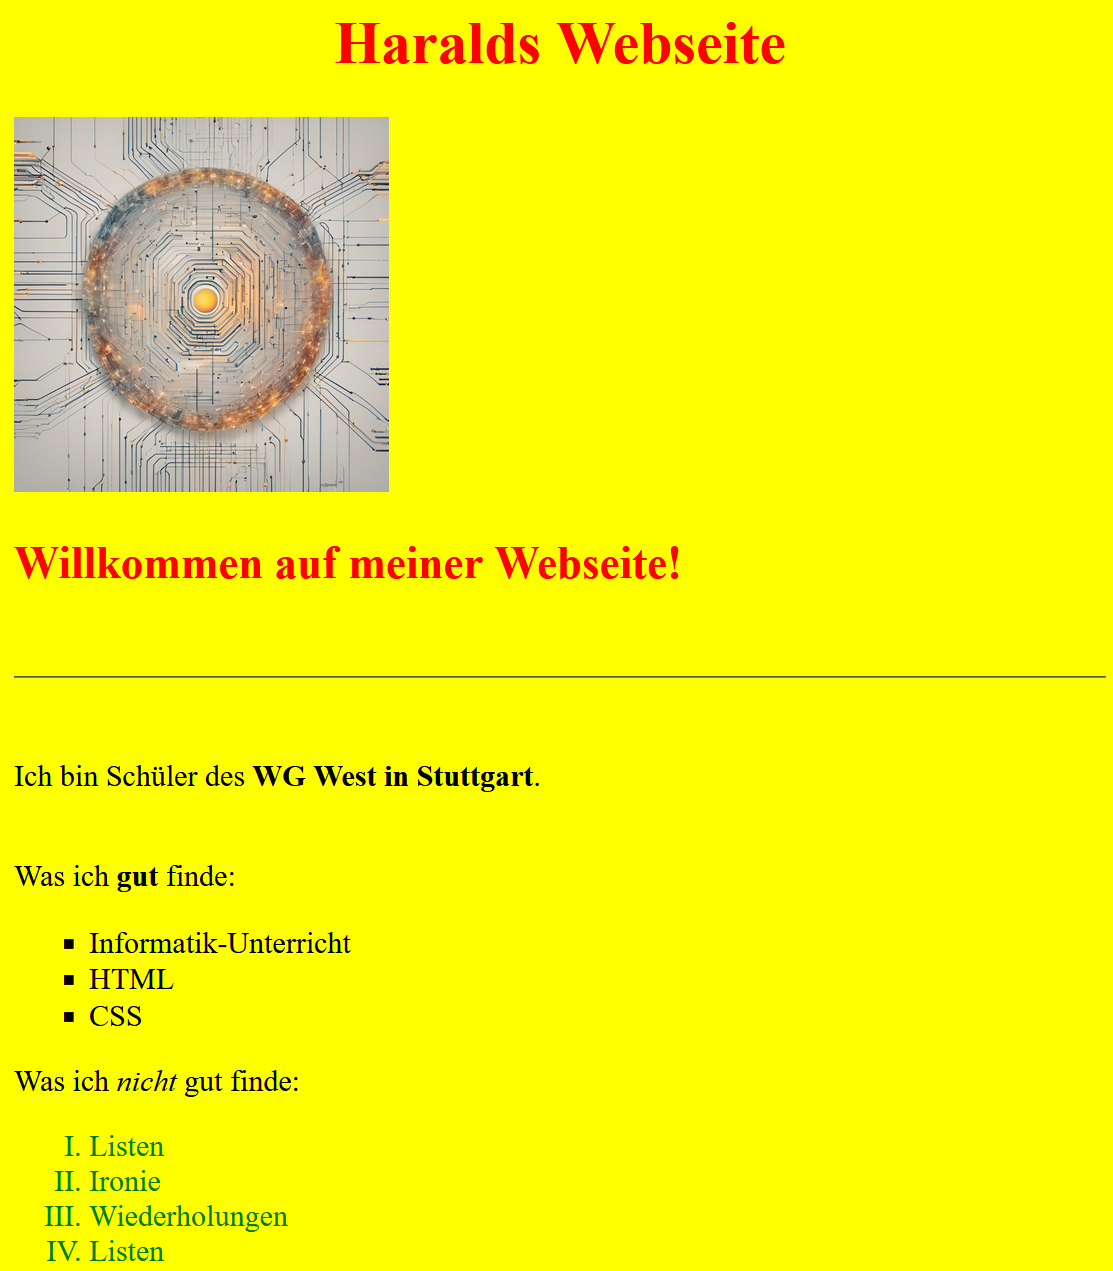
\includegraphics[width=\linewidth]{\pics/BilderEinfuegen.png}
\end{minipage}
\begin{Exercise}[title=, label=Bilder]
    \begin{enumerate}
        \item Lade dir ein Bild aus dem Internet herunter und speichere dieses in einem Ordner Bilder, der im gleichen Verzeichnis wie \textit{schueler.html} liegt. Kurze Dateinamen machen das Einbinden leichter.
        \item Binde in deiner \textit{schueler.html} das Bild ein. Recherchiere dazu den Tag für das Einfügen von Bildern. Erkundige dich, welche Attribute für die Höhen- und Breitenangabe von Bildern notwendig sind und was der Alternativtext bei Bildern bedeutet.
        \item Um ein Bild einzubinden, muss man einen Dateipfad angeben. Wie funktionieren relative und absolute Pfadangaben? Welche Vor- und Nachteile bieten die beiden Möglichkeiten?
    \end{enumerate}
    Informiere dich über die wesentlichen Bildformate (Rasterbilder wie jpg, gif, png oder Vektorgrafiken wie svg) und deren Unterschiede. Wichtige Begriffe sind hier unter anderem Dateigröße, Komprimierung, Transparenz, Farbraum.
\end{Exercise}


